\documentclass[10pt]{beamer}

\usetheme{Madrid}
\usecolortheme{default}
\setbeamertemplate{navigation symbols}{}
\setbeamertemplate{footline}[frame number]

\usepackage{amsmath, amssymb}
\usepackage{graphicx}
\usepackage{booktabs}
\usepackage{xcolor}
\usepackage{array}

\definecolor{hl}{RGB}{200,40,40}
\definecolor{accent}{RGB}{30,80,160}

\newcommand{\red}[1]{\textcolor{hl}{#1}}
\newcommand{\blue}[1]{\textcolor{accent}{#1}}

\title[Compositional RTL with LLM Agents]{Compositional RTL Design with LLM Agents\\[2pt]\large Multi-Model IP-Reuse Benchmark}
\author{Leonardo Ferreira \and Matthew Kotzbauer \and Warren Zhu}
\institute[Team 11]{Team 11 -- COMPSCI 1440R/2440R, Spring 2026 -- Final Presentation}
\date{April 27, 2026}

\begin{document}

% ------------------------------------------------------------
\begin{frame}
  \titlepage
\end{frame}

% ------------------------------------------------------------
\begin{frame}{Where we landed}
  \begin{itemize}
    \item Project framing (unchanged): \blue{IP reuse, not scratch generation}, is the part of chip design current LLMs are weakest at.
    \item Intermediate deliverable was a single harness on top of one LLM.
    \item HT's note: \emph{turn this into a benchmark; compare LLMs.}
    \item This deck: \red{10 frontier LLMs across 3 providers}, scored on IP routing against hand-labeled gold.
  \end{itemize}

  \vspace{0.5em}
  \footnotesize
  Scratch baseline kept as a foil. The interesting axis is whether bigger models actually pick the right IP, not whether they write better Verilog from scratch.
\end{frame}

% ------------------------------------------------------------
\begin{frame}{The eval (one slide, no architecture)}
  Pipeline per (LLM, problem):
  \vspace{0.3em}
  \begin{enumerate}
    \item Send the spec + planner system prompt to the LLM.
    \item Parse the JSON subblock list.
    \item For each \texttt{REUSE\_IP}-suggested block, run our MCP-backed router over the 20-IP corpus.
    \item Score against \blue{9 hand-labeled gold entries} on the ChipBench cpu\_ip set.
  \end{enumerate}

  \vspace{0.6em}
  Metrics:
  \begin{itemize}
    \item \textbf{Precision}: of the IPs the router picked, what fraction are in the gold set?
    \item \textbf{Recall}: of the gold IPs, what fraction did the router pick?
    \item \textbf{Kind agreement}: per planner subblock, does \texttt{REUSE\_IP} vs \texttt{GENERATE} match the gold label?
  \end{itemize}

  \vspace{0.4em}
  \footnotesize
  This is not pass-rate. A model can write perfect Verilog and still fail the routing eval if it never recognizes that an off-the-shelf register file is on the shelf.
\end{frame}

% ------------------------------------------------------------
\begin{frame}{Models tested}
  \begin{center}
  \begin{tabular}{lll}
    \toprule
    Provider & Model & Released \\
    \midrule
    Anthropic   & Claude Opus 4.7    & 2026-02 \\
    Anthropic   & Claude Sonnet 4.6  & 2025-12 \\
    Anthropic   & Claude Haiku 4.5   & 2025-10 \\
    OpenAI      & GPT-5.4            & 2026-03 \\
    OpenAI      & GPT-5.2            & 2025-12 \\
    OpenAI      & GPT-5.1            & 2025-11 \\
    OpenAI      & GPT-5              & 2025-08 \\
    OpenAI      & GPT-4.1            & 2025-04 \\
    AWS Bedrock & DeepSeek-R1        & 2025-01 \\
    AWS Bedrock & DeepSeek V3.2      & 2025-09 \\
    \bottomrule
  \end{tabular}
  \end{center}

  \vspace{0.6em}
  \footnotesize
  Same planner prompt across all 10 models. No few-shot examples. Same router (deterministic, MCP-backed). Same 20-IP corpus. Same 9 cpu\_ip problems.
\end{frame}

% ------------------------------------------------------------
\begin{frame}{Result 1: routing quality by LLM}
  \begin{center}
    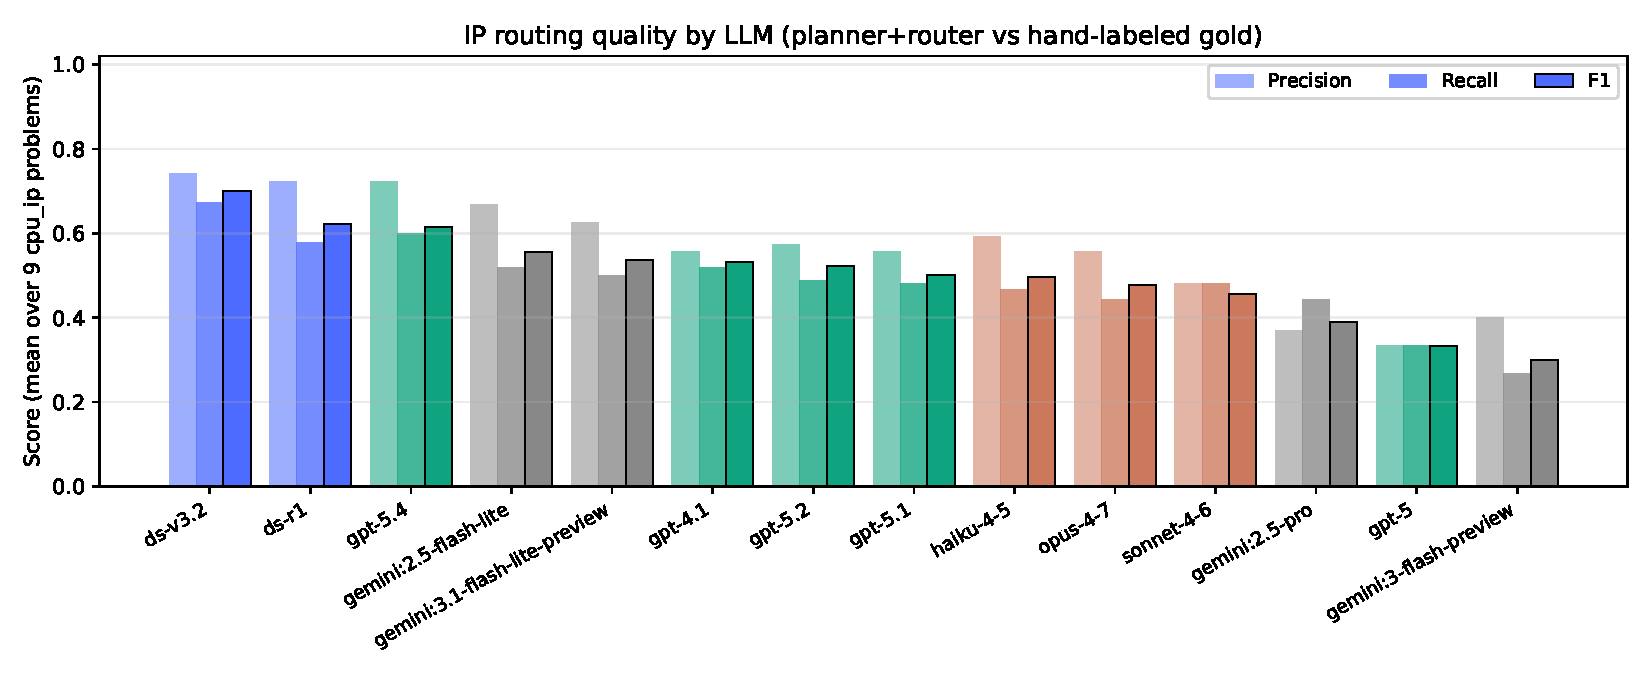
\includegraphics[width=0.95\linewidth]{figs/routing_f1.pdf}
  \end{center}

  \vspace{-0.3em}
  \footnotesize
  Mean over 9 cpu\_ip problems. Color = provider (green OpenAI, orange Anthropic, blue Bedrock).
\end{frame}

% ------------------------------------------------------------
\begin{frame}{Result 2: scratch baseline (foil)}
  \begin{center}
    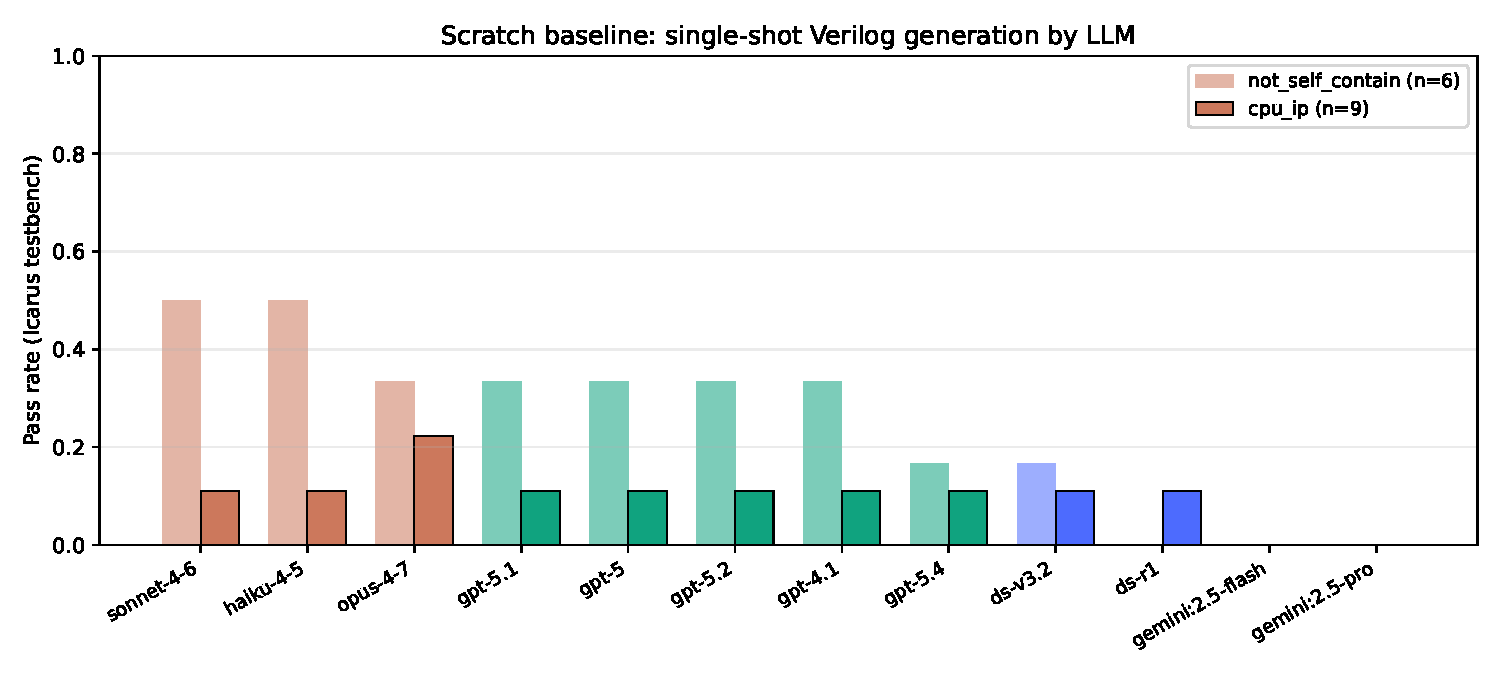
\includegraphics[width=0.95\linewidth]{figs/scratch_baseline.pdf}
  \end{center}

  \vspace{-0.3em}
  \footnotesize
  Pass rate is testbench-driven (Icarus). \texttt{not\_self\_contain} is hierarchical, \texttt{cpu\_ip} is RISC-V IP blocks.
\end{frame}

% ------------------------------------------------------------
\begin{frame}{Result 3: routing skill vs scratch skill}
  \begin{columns}[T]
    \begin{column}{0.55\linewidth}
      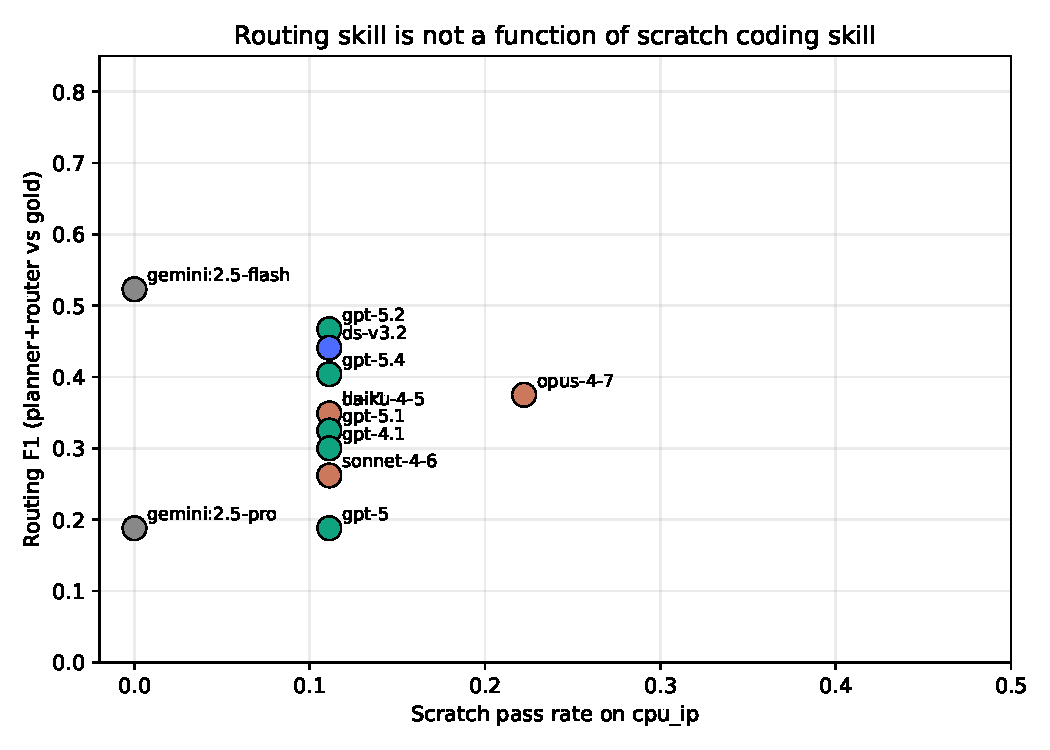
\includegraphics[width=\linewidth]{figs/routing_vs_scratch.pdf}
    \end{column}
    \begin{column}{0.45\linewidth}
      \footnotesize
      \begin{itemize}
        \item Routing F1 and scratch pass rate are \red{not the same axis}.
        \item Some strong scratch coders fail at routing. They re-author IP that was on the shelf.
        \item Some weaker scratch coders route well. They follow the planner prompt's structure.
        \item \blue{Implication}: a reuse-aware metric surfaces a capability that scratch benchmarks completely hide.
      \end{itemize}
    \end{column}
  \end{columns}
\end{frame}

% ------------------------------------------------------------
\begin{frame}{Failure modes we saw}
  \begin{itemize}
    \item \textbf{Hallucinated IP picks}: planner labels a 32-bit ALU as \texttt{REUSE\_IP}, router pulls \texttt{priority\_encoder}. Router only matches on search-query overlap; planner has to give it a usable query.
    \item \textbf{Over-decomposition}: weaker models split a 5-line spec into 6 subblocks, all \texttt{GENERATE}. Wastes budget; nothing reuses.
    \item \textbf{Under-decomposition}: stronger models sometimes return one big \texttt{GENERATE} block. Skips the corpus entirely.
    \item \textbf{Kind-flip}: same model on the same problem swings between \texttt{REUSE\_IP} and \texttt{GENERATE} across runs. Temperature 0; still happens.
  \end{itemize}

  \vspace{0.4em}
  \footnotesize
  None of these are LLM-skill problems in the usual sense. They're \blue{prompt-design and corpus-coverage} problems. That's a tractable place to push.
\end{frame}

% ------------------------------------------------------------
\begin{frame}{Takeaways}
  \begin{enumerate}
    \item \blue{IP-reuse skill is its own axis.} It does not track scratch pass rate. A multi-model eval surfaces that gap; single-model harness benchmarks hide it.
    \item \blue{The planner is the bottleneck, not the codegen.} Across 10 models, router behavior is deterministic; variance lives in subblock decomposition and \texttt{search\_query} quality.
    \item \blue{A 20-IP corpus is enough to score 9 cpu\_ip problems meaningfully.} Corpus depth matters more than corpus breadth at this scale.
  \end{enumerate}

  \vspace{0.6em}
  \textbf{Future work}
  \begin{itemize}
    \item Open the eval to community submissions. Same protocol, any model, any planner prompt.
    \item Reuse ratio on the integrated TopModule (LoC reused / total LoC), not just routing.
    \item Fine-tune a small open model (SiliconMind-style) on harness traces from the strongest planner.
  \end{itemize}
\end{frame}

% ------------------------------------------------------------
\begin{frame}{References}
  \footnotesize
  \textbf{Prior work}
  \begin{itemize}
    \item ChipGPT, VeriGen, RTLCoder -- scratch generation
    \item ChipNeMo (NVIDIA) -- domain-adapted chat / EDA
    \item HiVeGen (ICLAD '25) -- snippet retrieval, not IP reuse
    \item MAGE -- multi-agent decomposition, scratch per subtask
    \item SiliconMind-V1 -- our base architecture
  \end{itemize}

  \textbf{Benchmarks}
  \begin{itemize}
    \item ChipBench (UCSD/Columbia '26) -- problems we score on
    \item VerilogEval (NVIDIA), RealBench
  \end{itemize}

  \textbf{Open IP corpora used in plan}
  \begin{itemize}
    \item OpenTitan (lowRISC), PULP common cells, Adapteva OH!, Forencich UART/I2C/AXI/Ethernet, dawsonjon FPU
  \end{itemize}

  \vspace{0.5em}
  \textbf{Code}: \texttt{github.com/MattKotzbauer/rtl-mosaic}
\end{frame}

\end{document}
